\documentclass{article}

\author{Philip Hale}
\title{Natural Language Processing: Assessment 2}

\usepackage{graphicx}
\usepackage{epstopdf}
\usepackage{minted}

\begin{document}

\maketitle

\section{Task 1: Grammar development – 50\%}

\begin{figure}
  \centering
  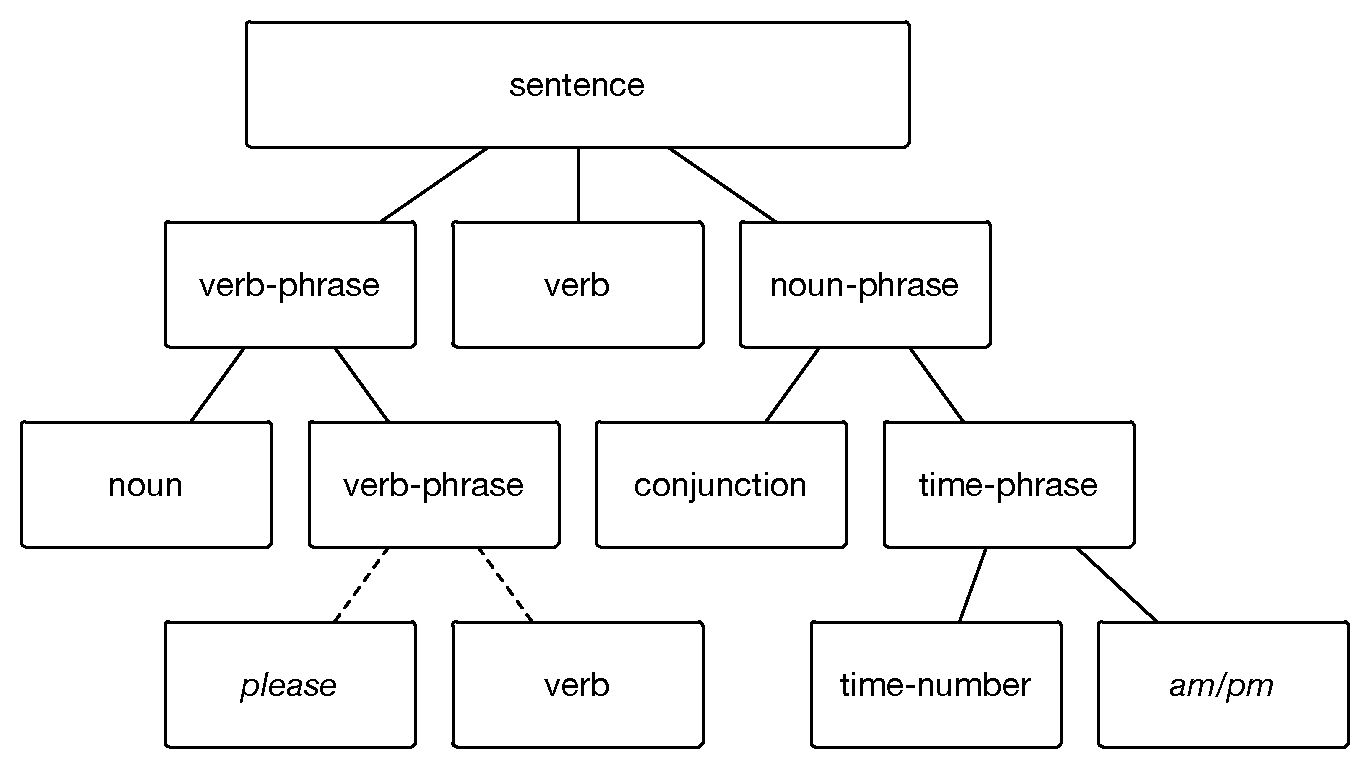
\includegraphics[width=\textwidth]{dcg_grammar.eps}
  \caption{DCG Grammar}
  \label{fig:dcg_grammar}
\end{figure}

See Figure~\ref{fig:dcg_grammar} for a graphical representation of the following
DCG grammar:

\begin{minted}{prolog}
sentence --> noun_phrase, verb_phrase.
noun_phrase --> det, noun.
verb_phrase --> verb, noun_phrase.
det --> [the].
det --> [a].
noun --> [cat].
noun --> [bat].
verb --> [eats].
\end{minted}




\section{Task 2: Semantic interpretation – 30\%}

\section{Task 3: Discussion of the approach – 20\%}

\end{document}

